% !TeX root = ./main.tex
\documentclass[a4paper, 12pt]{article}
\usepackage[margin=2.5cm]{geometry}
\usepackage{parskip}
\setlength{\parindent}{1cm}
\setlength{\parskip}{6pt}
\usepackage{glossaries}
\usepackage{listings}
\usepackage{color}
\definecolor{lightgray}{rgb}{.9,.9,.9}
\definecolor{darkgray}{rgb}{.4,.4,.4}
\definecolor{purple}{rgb}{0.65, 0.12, 0.82}
\lstdefinelanguage{JavaScript}{
  keywords={break, case, catch, continue, debugger, default, delete, do, else, false, finally, for, function, if, in, instanceof, new, null, return, switch, this, throw, true, try, typeof, var, void, while, with},
  morecomment=[l]{//},
  morecomment=[s]{/*}{*/},
  morestring=[b]',
  morestring=[b]",
  ndkeywords={class, export, boolean, throw, implements, import, this},
  keywordstyle=\color{blue}\bfseries,
  ndkeywordstyle=\color{darkgray}\bfseries,
  identifierstyle=\color{black},
  commentstyle=\color{purple}\ttfamily,
  stringstyle=\color{red}\ttfamily,
  sensitive=true
}

\lstset{
   language=JavaScript,
   backgroundcolor=\color{lightgray},
   extendedchars=true,
   basicstyle=\footnotesize\ttfamily,
   showstringspaces=false,
   showspaces=false,
   numbers=left,
   numberstyle=\footnotesize,
   numbersep=9pt,
   tabsize=2,
   breaklines=true,
   showtabs=false,
   captionpos=b
}

\makeglossaries

\title{\Large{\textbf{Student Wellbeing Project}}}
\author{By Tarnjot Virdee}
\date{29th April 2019}

\begin{document}

\maketitle
\clearpage
\tableofcontents
\clearpage

\section{Introduction}

My Introduction thing
My Introduction thing
My Introduction thing
My Introduction thing
My Introduction thing
My Introduction thing
My Introduction thing
My Introduction thing
My Introduction thing
My Introduction thing
\section{Problem Articulation and Objectives}
% Describe the problem, have plateau as is and plateau to be.
% Flow diagrams or something, describe what is wrong with the current process and propose a high level view of what the
% plateau/system to be is.

\subsection{Problem statement} \label{problemstatement}

% Introduction to the problem
Pressures from University life can cause a number of health issues in students.
In some cases students may experience stress attributed to not understanding topic and meeting deadlines.
Such an environment can also act as a catalyst for those that are already experiencing other issues outside of University.
Those that do not find themselves with the appropriate support may not have the confidence to engage the initiative to arrange help sessions 
with their General Practitioner (GP) or any on-campus support groups. 
A recent report has stated that 95\% teens in 2018 either have access or own a smartphone device \cite{monicajing2018teenstechnology}.
This is the same group of people from which 15\% to 20\% suffer from mental health issues.
Taking both of these facts into account, an effort can be made to utilise the smartphone that exist in pockets of almost all these people 
and provide an anonymous way to start figuring out issues related to their own wellbeing.


\subsection{Project scope}
This scope of this project is to create a prototype, covering some of the necessary groundwork, in how a chosen set of technologies can be used 
to solve the issues raised in the problem statement (\ref{problemstatement}).

\subsection{Solution-as-is}
% Discuss the plateau-as-is/solution-as-is, identifying why it's not ideal.
Though many survey tools are available on the market, that are free to use, none have be tailored to address student wellbeing concerns.
Applications that are available, such as Google Surveys and Survey Monkey, are generic survey creation tools that can be shared with 
people via email or a link.
It makes sense that these online solutions are generic as they are aimed to cover as many use cases as possible.
This abstract approach to creating surveys is unlikely to be the ideal approach for specific issues around a single topic; such as
student well-being.
It is difficult to direct students to the appropriate resources, depending on the way they answered, as this type of functionality is not
provided by existing tools.
This project aims to create a web application that can be used across all devices and allow surveys to be created and pushed to students.
It would be useful, to students, to have an application that can produce a score from completing a set of surveys and be directed to relevant
resources specific to them.

\subsection{Stakeholders}

\subsubsection*{Students}
Students are one of the main stakeholders due to this system revolving around those that are suffering for poor mental health.
Feedback from students will be vital for the software solution to be a success.

\subsubsection*{Mental health experts}
Experts will have a keen interest in the proposed software solution as the system will be tailored to allow such users to easily

\subsubsection*{Lecturers/University staff}
Those that lecture students, along with other personnel at a university, are likely to have an interest in the effectiveness of the software solution.
If the effects on student performance is tangible, in some metric the university uses, then they would likely want to promote its use among students.

\subsection{Assumptions}
For development purposes, it makes sense to lay out some assumptions for the proposed software solution as a means to provide focus throughout the development process.

\begin{itemize}
    \tightlist
    \item Only health experts will be creating surveys
    \item Only students will be responding to surveys
    \item Only university students will be using this system
    \item A web application and android application are the only platforms that are used
    \item There will be one account per user type
    \begin{itemize}
        \item One for student
        \item One for expert
    \end{itemize}
\end{itemize}


\subsection{Constraints}

\subsubsection*{Only one developer}
The main constraint to take into consideration is that there will only be a single developer working on this project throughout the year.
This limitation means that development will take much longer than it typically would in a regular team of software engineers.

\subsubsection*{Technical limitations}
The developer will need to learn many technologies along the way as they have never developed a web application before.

\subsubsection*{Limited time}
Due to there being a seven to eight month time constraint, it is highly likely that only an initial prototype will be achievable.
This constraint also means that there is a chance that not all the desired features will be implemented by the deadline. 


\subsection{Technical specification}
The project initiation document (PID) specified the functionality that is required by the software solution and this has not changed as of writing this report.
Minor changes have been made to what was initially specified in the PID due to the feasibility involved.

\begin{itemize}
    \tightlist
    \item Server-side application
    \begin{itemize}
        \item Managing databases
        \item Providing an Application Programming Interface (API) to allow a client to modify data in the underlying databases
        \item Runs multiple small services for managing and processing data (microservices)
    \end{itemize}

    \item Web-based application (client-side)
    \begin{itemize}
        \item Allows for experts and students to \emph{log in} and access the relevant features from a web browser environment
        \item User components that can be re-used when developing the android application which will allow for a more unified user experience
    \end{itemize}

    \item Android application (client-side)
    \begin{itemize}
        \item Allows for experts and students to \emph{log in} and access the relevant features from an android application running on a mobile device 
        \item Android application will mostly be tarted for running on mobile phones rather than tablets as most users carry around a smartphone rather than a tablet device
    \end{itemize}

    \item Experts must be able to:
    \begin{itemize}
        \item Create surveys via some sort of interface on one of the client applications (web or android)
        \item Have a way to direct subscribed to students to some sort of help depending on said student's responses to a survey 
        \item Collect survey data and be able to visualise it 
    \end{itemize}
\end{itemize}

\subsection{Motivation model}
% Based on all the points covered so far, the following motivational model can be drawn out.
A motivational model can be drawn out as a way to present the breakdown of the problem domain.
The elements on the left hand side of figure \ref{motivationmodel} address the existing architecture, the right hand side addresses the desired
architecture for the system to be implemented.
Each system represented in the figure is a specialisation of an overall problem domain so are represented as such.

\begin{figure}[H]
    \centering
    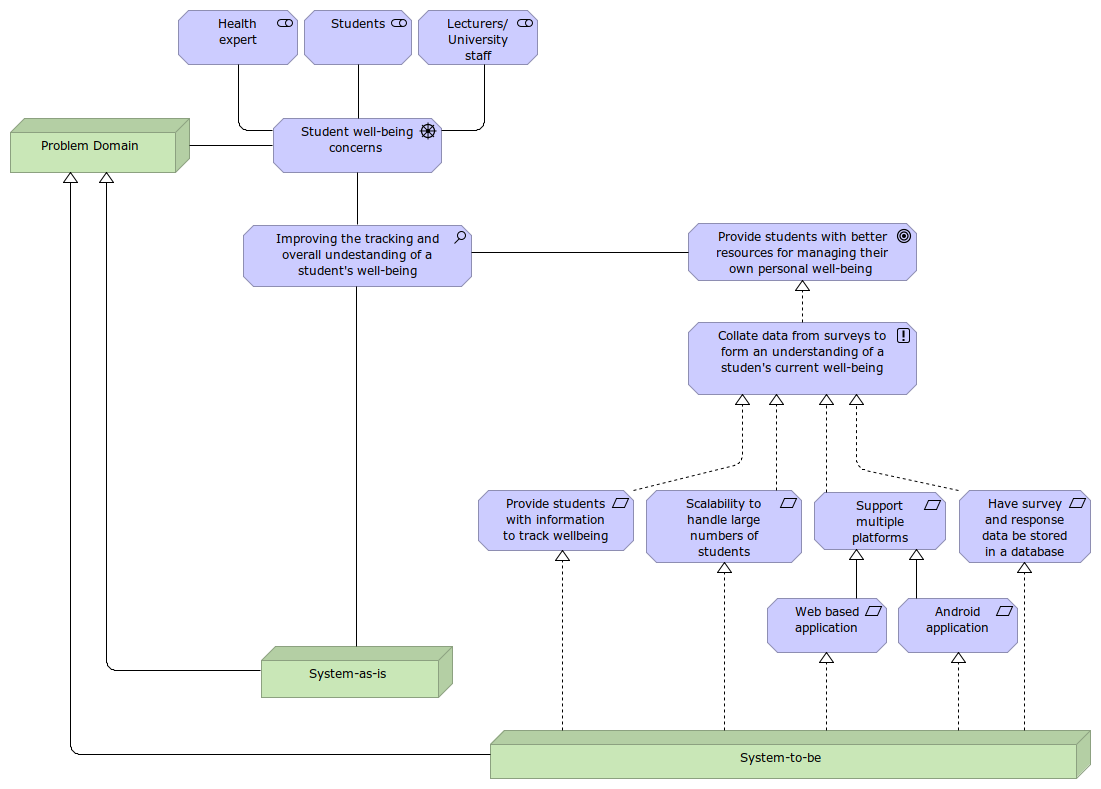
\includegraphics[width=350px]{images/motivation_model.png}
    \caption{Motivation model derived from the initial brief}
    \label{motivationmodel}
\end{figure}

\subsection{Solution-to-be}

\begin{figure}[H]
    \centering
    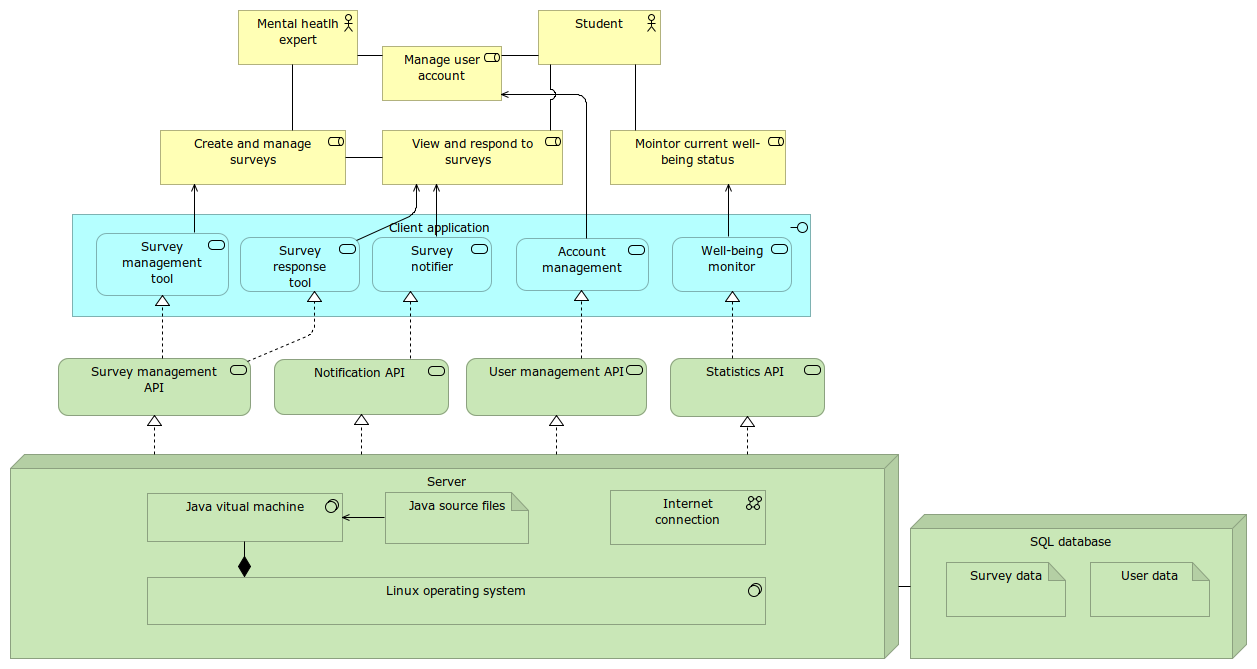
\includegraphics[width=350px]{images/solution-to-be.png}
    \caption{Proposed system solution}
    \label{solutiontobe}
\end{figure}


% Discuss the plateau-to-be/solution-to-be, specifying why it would be a good solution to the current issues with the available things already.
% The aim of this project is to provide a solution that is tailored for measuring student wellbeing. 
% In order to do this, there are some key features that need to be implemented.
For this solution to be effective, the survey creation tool needs to allow an \emph{expert} to create a survey with answers that have 
a weighted score associated with it. 
Being able to calculate an overall score allows users, both the creator and student that answered the survey, to understand the level of 
wellbeing that the student is at; identifying potential issues that may need to be addressed.
Understanding what potential issues could be present can allow a survey creator to specify resources for different scoring thresholds.
Just like other solutions, a web application would be the ideal approach as it will allow it to be used across all platforms through a web
browser.
An android application would be ideal to include, as a part of this solution, as it can allow notifications to be pushed to devices; allowing
users to know when a new survey is available to participate in.
Displaying analytic data to students, based on survey responses, can allow them to have a better way of monitoring their wellbeing.
It can also facilitate a way for people to compare their scores, and wellbeing status, with other users if they choose to as user data should be
anonymous by default.all the points covered so far, the following motivational model can be drawn out.

\section{Literature Review}

In the early stages of this project research was conducted of existing literature and technologies to grasp a better understanding of the problem and what would be the best approach to solve it.
This section will cover the main areas that this project will focus on.

\subsection{Wellbeing of university students}

Since this report revolves around the topic of student wellbeing, it is important to establish a definition for the term "student wellbeing" to correctly approach the problem.
It is defined as a sustainable state of positive mood and attitude, resilience, and satisfaction with self, relationships and experiences at school \cite{noble2008scoping}.
The part referring to a sustainable state is important to focus on. All humans endure fluctuations their emotional state within their lives, but a real problem occurs when their emotional state is not sustainable.
There are many factors that can play into poor mental health. Stress tends to be one of the main issues. 
Stress arouses feelings of fear, incompetence, uselessness, anger and guilt \cite{turunen2014indoor}, it can be expected that this will lead to behavioural changes. 
To some, these attributes that stem from stress can act as a form of motivation, however not all are able to do such a thing.
Those that are unable to cope with stresses from university studies will, unfortunately, struggle to focus on assignments and revision for exams.
A study by HSBC, found a correlation between disadvantaged social circumstances with increased health risks \cite{currie2009social}.
While talking about students, it is important to recognise that there may be deeper stemmed issues within the lives of certain students that may affect them when entering higher education.

Most disorders that pertain to mental health first start developing between the ages of 15 and 20 years of age \cite{kessler2005lifetime}.
By taking this fact into account, 15\% to 20\% of individuals who fall into this category (youth \cite{youth2017definition}) are affect by some sort of mental disorder; the majority whom suffer from an anxiety order. 
The study, conducted by The university Of British Columbia, therefore came an approximate figure of 140,000 children and youth who suffer from a mental disorder. 
UCAS have reported that, on average across the United Kingdom, that 27\% of people aged 18 years old had been accepted into universities \cite{ucas_2018}.
This percentage makes up a total of 353,960 students. 
After applying the 15\% estimate, there are likely around 53,000 students that are starting their university life, in 2018, with undiagnosed mental health problems.

Stigmas/stereotypes associated with having such a condition are accepted in western societies \cite{corrigan2002paradox}.
By acknowledging this, one can understand how it is difficult for these individuals to engage in constructive discussions.
Anonymising feedback for those that wish to get help without anybody judging would be a good place to start. 

\subsection{What makes a good survey creation tool?}

The main objective of this project is to provide the necessary tools for health experts to curate surveys for students to respond to.
Data from completed surveys can be used to direct students to appropriate resources depending on choices for each question.


\subsection{Web-app architectures}
In the world of software engineering, there are many approaches to solve a single problem.
Throughout the years, along with the evolution of technology, approaches have changed to ensure that products are
can be developed and maintained in a manner and time that allows businesses to adapt and react to ever changing markets. 
One of the main concerns of a business is to grow [citation], this is why having an architecture in place that is scalable is
critical to maintain a competitive edge and meet the demands of customers.

There are common architecture approaches used when developing a web application.
A recent article by Microsoft listed approaches typically taken as of 2019. 
Monolithic and n-layer approaches are the typical avenues taken by software developers in recent years \cite{ardalis_common}.
An architecture model is chosen based on what is required and how quickly an application needs to be developed.

\subsubsection{Monolithic}
Monolith applications is one that is entirely self-contained, in terms of its behaviour \cite{ardalis_common}.
It may interact with other services or data stores, but the core functionality is shipped as a single unit.

The main motivation for wanting to deploy an application built this way is how it is easier to deploy \cite{namiot2014micro}.
Issues arise with this approach is when new features need to be added. The need to grow the feature set of an application likely means
more developers need to be recruited. A large, intertwined, codebase generally requires new recruits to spend a lot more time learning
how the existing codebase functions and understand how to correctly implement new code that does not compromise the existing stability.
A lot of communication will be required by a team, while developing features, to ensure compatibility.
This results in a lot of wasted time as it fundamentally compromises productivity and may result in poor quality code to meet deadlines.
In order to scale such an application, the only clear approach would be to run multiple instances of it behind a load balancer.
This is a very inflexible way to adapt to growing demand for a service.
Due to how multiple instances of the same application will be required, the resources required will also need to scale at the same rate.
For large companies, this is just un-feasible due to the costs for either buying or renting the resources. 

Ideally monolith application should only be used while developing initial prototypes. If they are to be deployed in production environments,
it should really only be for very small client bases that are unlikely to need extensive scaling.

\subsubsection{N-layer}

Modern web architectures, in production environments, typically adopt a three tier approach which is a client-server architecture approach.
This approach to software design allows presentation, data processing and data storage functionalities to be separated.
A result of this is that three distinct layers to the project can be worked on independently from one another; even separate teams for
each product layer. 

Less learning will be required for new recruits due to less code, compared with a monolith codebase, needing to be learned.
Scaling an application that utilises a layered architecture approach would be a lot easier to scale due to the independence of each layer.

\subsection{Presentation layer (front-end) technologies}
A user interface for a web based application is found as part of the presentation layer.
This front end application will rely heavily on the need to send and receive requests from a server application (application layer) as 
it drives the core business functions.
As it is an application, technologies that allow for dynamic interactions with the web page are required.

HTML (Hyper Text Markup Language) with CSS (Cascading Style Sheets) are core technologies for building web pages \cite{w3c_html_css}.
Structure of a web page is defined by HTML whereas styling and layout is defined by the CSS used.
Web applications need to enable interactivity with the end user; HTML and CSS alone cannot achieve this.
Javascript is predominately used to provide dynamic behaviour and is based off the ECMAScript standard \cite{stefanov2010javascript}.
Through the large amount of support Javascript has had over the years, a number of frameworks and libraries have come about.
A focus will be made on three of the most popular tools for creating professional user interfaces; Angular, React and Vue \cite{stateofjs_2018}.

\subsubsection{W3C Document Object Model (DOM)}
It is important to define what DOM is before discussing JavaScript frameworks and technologies due to the reliance on the manipulation of the DOM to 
create dynamic web pages that users can interact with.
DOM is a W3C standard that defines a language and platform-neutral application programming interface (API) for accessing, navigating, and 
manipulation of HTML and XML documents.
It defines the logical structure of documents and the way a document is accessed and manipulated \cite{wood1999programming}.
The main benefit of the DOM is the way it allows programmers to build documents, navigate its structure and manipulate elements on that page.
JavaScript allows web pages to become dynamic as it facilitates the, on the fly, manipulation of the DOM for a HTML document.

\subsubsection{Angular}
Angular is a JavaScript MVC framework created by Google to properly architecture and maintain web applications.
It embraces extending HTML into a more expressive and readable format. 
Since Angular is built and maintained by Google, there is a large community available that developers can learn from.
Angular evaluates the markup of a HTML document only after it has been loaded into the DOM.
This approach brings about three key benefits.

As stated, Angular only starts evaluating a page after the main loading process has been completed.
The main advantage of this is that it allows developers to start implementing Angular code into existing pages.
Since Angular is completely rendered on the client-side, it removes the need for any server or build process. 
If code has been added into a HTML page, it can be opened up into a browser and have scripts be executed straight away.
Extensibility is another great feature of Angular where the option to create custom elements is available for developers.
Developers can also define how an element is rendered and assign behaviours to it; allowing custom libraries to be built \cite{jain2015angularjs}.

\subsubsection{React} 
React was originally created by engineers at Facebook to solve the challenges involved when developing complex user interfaces with datasets 
that change over time \cite{gackenheimer2015introduction}. 
Unlike Angular, which is a framework, React is a library of tools that developers can use to create interactive pages.
Developers, over the years, have wanted to get away from directly interacting with the DOM due to how unfriendly it was for many.
The aim of React is to avoid this direct interaction with the DOM and instead deal with a virtual DOM that abstracts away from
the real one. This approach greatly simplifies the programming model involved while improving performance \cite{staff2016react}.

A big problem Facebook faced was keeping the user interface in sync with both the business logic and the state of the application.
Normally you would have to use a centralised event bus, by putting events into the queue or by having listeners for the event that would then go
ahead and make the necessary changes to a page. 
For programmers, this was overly cumbersome. Hence the desire to innovate to solve this problem.
React applications are able to automatically re-render themselves when there has been a change to the underlying data model.
A diff (comparison between before and after) is conducted to observe what has actually changed. The components that have exhibited a change are the
only ones to get re-rendered \cite{staff2016react}.
 
An extension to React, for creating native mobile applications, is called React Native. Unlike ReactJS, which is a JavaScript library,
React Native is a framework. 
This framework is based on ReactJS, but instead of targeting a browser application, it targets mobile platforms.
The idea behind this is to allow developers to write, fluid, native applications from the comfort and familiarity of an established library.
Code can be shared between platforms; making it easy to develop for both iOS and Android \cite{eisenman2015learning}.

\subsubsection{Vue}
Created by Evan You, Vue was created out of the need to quickly prototype a large user interface.
Rather than writing out a lot of repeated HTML, there was a desire to find a framework or tool that may already exists that solves the exact problem Evan had.
At that time Angular was widely used and React had only started. As great as these technologies were at the time, they were not flexible and lightweight
enough for fast prototyping of user interfaces. Though Vue started off as a tool for fast prototyping, it has matured over the
years to become something developers can use to build complex, scalable and reactive web pages \cite{filipova2016learning}.
The core library, for Vue, is focused on the view layer only, and is very easy to pick up and integrate with other libraries or existing projects \cite{koetsier2016evaluation}.
Similarities can be drawn to React where both use a virtual DOM and have components that can be reused.

https://vuejs.org/v2/guide/comparison.html comparisons between React and Vue from official Vue website.


\subsection{Web services API} \label{web services}
An API (application programming interface) that allows two independent components of an application to communicate with one another.
SOAP and REST are two widely used technologies that are used when developing a web services API.

\subsubsection{Web 2.0}
Before being able to understand why SOAP and REST have come about, it is important for the reader to have a basic understanding what is meant by Web 2.0 and how it.
The term has been around since 2005 but has been a controversial subject. It has mostly been controversial due to a lack of agreement on what exactly is meant
by the term \cite{constantinides2008web}. For the purposes of this paper, the following definition from Techopedia will be used:
\begin{quotation}
    \textit{
        Web 2.0 is the name used to the describe the second generation of the world wide web, where it moved static HTML pages to a more interactive and 
        dynamic web experience.
        Web 2.0 is focused on the ability for people to collaborate and share information online via social media, blogging and Web-based
    }
    \cite{web2definition}. 
    
\end{quotation} 

\subsubsection{SOAP}
SOAP (Simple Object Access Protocol) is a lightweight protocol for exchange of information in a decentralised, distributed environment.
It is, exclusively, an XML based protocol and has three distinct parts to it: an envelope defining a framework for what is in a message and how to process it, 
a set of encoding rules for expressing instances of application-defined datatypes, and a convention for representing remove procedure calls and responses \cite{box2000simple}.
Version 1.1 of SOAP specification, published on 8 May 2000, did not pass W3C recommendation status. It was only 24 June 2003 that it finally became a W3C recommendation;
making it accepted as an industry standard. 

\subsubsection{REST}
REST (Representational State Transfer) is a pattern of resource operations that has emerged as the standard for service service design in Web 2.0 applications.
REST’s simplicity, along with its natural fit over HTTP, has contributed to its status as a method of choice for Web 2.0 applications.
to expose their data. 
Resources in a RESTful service are both identified by and resolved with a URL \cite{battle2008bridging}.
The typical form you would see a URL in is: 

\begin{quotation}
    http://localhost:8080/Host/ApplicationPath/ResourceType/ResourceID
\end{quotation}

The core of any REST based design are CRUD (Create Read Update Delete) operations to deal with data stored on system.
In order to perform CRUD operations, REST utilises HTTP requests POST, GET, PUT and DELETE.
A great benefit of REST-based web design is the ability to use HTTP Headers to provide request context around each of theCRUD operations.
A request to a particular resource might result in HTML, XML, or JSON (compared to exclusively using XML with SOAP) depending on the desired
media type transmitted in the HTTP Accept header \cite{battle2008bridging}.

% Table to show a simple representation between CRUD to HTTP requests...
\begin{table} [h]
    \begin{center}
        \begin{tabular}{ |l|l|l| }
            \hline
            CRUD Operation & HTTP Request & Response format\\
            \hline
            Create & POST & 201 CREATED\\ 
            Read & GET & Determined by request headers\\  
            Update & PUT & 200 OK \\   
            Delete & DELETE & 200 OK \\
            \hline
        \end{tabular}
        \caption{CRUD operation to HTTP request mapping}
    \end{center}           
\end{table}

\subsection{Application layer (back-end) technologies}
The application layer is where all business logic would occur and facilitates features of an application.
Majority of the time, applications will be required to store data produced by end users. A data store, typically a database, is
used to do this.
In order for a front end component of the application to request data from the application layer, an API(application programming interface) needs
to be provided. The API provided, is what will allow the client-side JavaScript application to ``plug'' into the server to provide the business
logic. 
Modern web applications (Web 2.0), as discussed in section \ref{web services}, adopt REST as the standard way providing an API that can be used
by client-side applications.


This section will cover some technologies that are commonly used in industry to create the application layer for a web application.

\subsubsection{NodeJS}
NodeJS is a server-side JavaScript environment. It is based on Google's runtime implementation called the ``V8'' engine.
V8 and Node are mostly implemented in C and C++, allowing for high-performance runtime with low memory usage.
The difference between V8 and Node is where V8 mainly supports JavaScript in the browser, Node aims to support long-running 
server processes \cite{tilkov2010node}.
As an asynchronous event driven JavaScript runtime, Node is designed to build scalable network applications. 
Upon each connection the callback is fired, but if there is no work to be done, Node will sleep; freeing resources \cite{nodejs2016}.

One of the key advantages that NodeJS has over other solutions is the way it handles I/O.
Servers that implement multi-threading dedicate a thread to each browser connection in an attempt to prevent blocking calls being made \cite{frees2015place}.
Blocking is when the execution of additional JavaScript in the Node.js process must wait until a non-JavaScript operation completes \cite{nodejs2019blocking}. 
Managing resources can be challenging with this approach, especially when dealing with a large number of connections.
NodeJS only runs on a single thread and deals with the blocking issue by exposing asynchronous APIs.
Asynchronous operations are generally a ``fire and forget'' type of operation; the reason why it solves the issue of blocking.
Node Package Manager (NPM) has also been a key tool in increasing the popularity of NodeJS.
In 2017, NPM had been reported to have over 350,000 packages \cite{linux2016stateofnpm}; demonstrating how active the community is.

A simple HTTP server is very easy to create; only taking a few lines of code to get running. 
This type of simplicity that NodeJS provides a more productive environment for developers as there is little configuration to do;
especially when developing initial prototypes.

\begin{figure}[htb]
    \begin{lstlisting}[language=JavaScript]
    var http = require("http")

    /* Create a server that returns a basic html response
     * Runs on localhost on port 3000 */
    http.createServer(function(req, res){
        res.writeHead(200, {'Content-Type': 'text/html'});
        res.end("<!doctype html><html><body><p>Hello World!</p></body></html>");
    }).listen(3000, "127.0.0.1");
    \end{lstlisting}
    \caption{Simple NodeJS HTTP server listening on port 3000}
\end{figure}
Though NodeJS has strong benefits, there are many problems surrounding it that prevent it being used more widely in industry.
Due to the single threaded nature, performance is poor when performing CPU intensive operations.
Several simple tasks (such as read/write database queries) can be queued in the background without blocking the main thread while
maintain fast execution speed. 

Due to the asynchronous nature of JavaScript, NodeJS relies heavily on callbacks to know when an operation has completed.
The term "callback hell" is prominent in the JavaScript community due to cumbersome nature of having to deal with them \cite{altexsoftnodejs}.
An example developers face, is to do with error-handling. The built in try/catch mechanism does network with asynchronous callbacks \cite{gallaba2015don}.
Instead workarounds are used to address issues such as this and are taken as a standard approach for performing such actions.
For developers that are used writing code that executes on multiple threads in a synchronous fashion, it can be difficult for them to
develop with asynchronous calls in mind.

\subsubsection{Java Spring Framework}
%Advantages, disadvantages, basic overview of features
Java Spring Framework/SpringBoot stuff here.

\begin{enumerate}
    \item fast
    \item can implement multithreading if required
    \item Supports everything node js does; async is available in Java
    \item mature set of tools that are tried and tested over the years; standards in place.
    \item lots of support
    \item biggest drawback being that there is a lot of configuration involved in Java
    \item But that's where springboot comes in and solves the problem; can get a server running very quickly
    \item Is a lot more verbose than than nodejs. More like C/C++ with statically typed code.
    \item Probably uses more resources
    \item Spring is more secure, lots of security options available to developers.
\end{enumerate}


\subsection{Data layer technologies}
Section talking about different ways to store data and discussing the different database types
that will allow someone to store this data. Talk about relational and non-relational databases and
state why one is better than the other. You don't have to come to a conclusion here, just discuss
the different options.


\subsection{Security concerns}

Can do a section with regards to security concerns such as SQL Injection and other vulnerabilities.
Can reference this later when arguing why using the technologies that you have are the best choice.
Sub section to do with web security.
\begin{enumerate}
    \item HTTPS, SSL, TLS
    \item Oauth2 or just to do with signing in stuff.
    \item JWT
    \item Sessions
    \item Possibly explore other common vulnerabilities in the web
\end{enumerate}
\section{Solution Approach}
The software solution is going to be a web application that connects to some sort of data storage.
In the modern web, there are many different approaches developers can take for creating scalable web applications.
An \textit{n-layered} architecture approach will be taken as this can provide the most flexibility for future scalability 
due to how vertical (more compute resources) or horizontal (more instances) scaling can be performed at each layer.

The 3 layer approach, typically used in industry, will be used for this project.
A presentation layer, application layer and data layer will therefore have to be created.

\subsection{Presentation layer}
Talking about how ReactJS is going to be used.
Also mention how React is just a library, it should be easy to port over the code to Android to build a native
android application that is consistent in design with the main web application.


\subsection{Application layer}
Functionality of the presentation layer will be dependant on the requests made to the application layer.
An application programming interface (API) will need to be exposed to provide that desired functionality.
As a modern web application, a set of RESTful API endpoints will be created.
The Java Spring Framework will be used to create a library of RESTful API endpoints for managing the contents of a connected database.


\subsubsection{Gradle}
Gradle is an open-source build automation tool for Java, just like Apache Maven, and was initially release in 2007 \cite{muschko2014gradle}.
Considering the vast number of dependencies available for Java, a built tool such as Gradle makes it much easier to bring in
a variety of different open-source components.
The idea behind Gradle was to take the best aspects of existing tools, such as Apache Ant and Maven, and improve on them.
Gradle is JVM native which allows for developers to write plugins and scripts with Java or Groovy; whichever is more convenient. 

\subsubsection{Springboot}

Stuff to do with springboot 

\subsubsection{REST API endpoints}

Stuff to do with rest api endpoints.


\subsection{Data layer}

Talk about the use of a relational database and include details about the initial approach to the schema.
\section{Design and Implementation}

At this point the project has a set of requirements to meet and basic solution approach has been outlined for each aspect of 
the project.
This section aims to inform the reader of the detailed design choices made and how this was implemented to achieve the final product.

\subsection{System model design}

\begin{figure}[ht]
    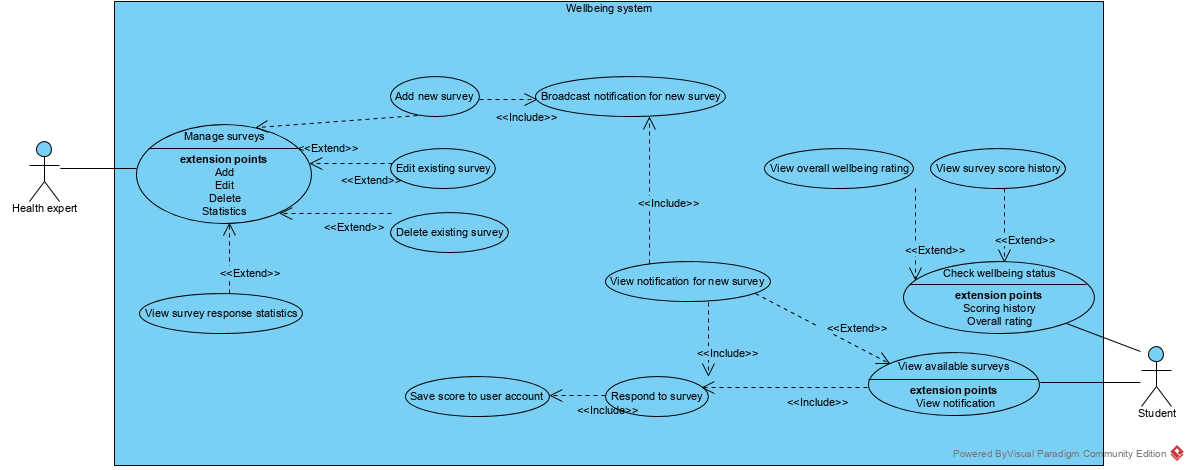
\includegraphics[width=450px]{images/system_model.png}
    \caption{Proposed system model}
\end{figure}


The proposed system model outlines the method in which an \textit{expert} can create, edit or delete a survey and how this can be 
fed to a student.
The main functionality to point out, that really links the two user types together, is how new survey send some sort notification 
to a (potentially) subscribed student; leading them to respond to the survey.
From the diagram, the reader should be able to see how a student will be able to either view surveys at their own will or be prompted
by a notification that had been sent out by some service.
The system outlines that there are really only two different categories of user that will use the system, this makes sense when looking
back at the articulation of the problem and the original brief given.

\subsection{Flow diagram}

An important process for the software solution is to be able to add and modify surveys for students to respond to.
The system model design does not go into much detail about this part of the system so it will be important to gain some clarity around this area.
Below is the proposed process flow diagram for what will occur when a user, of the system, attempts to add a new survey.
It outlines the need for authorisation (have permission to access such a resource) before carrying out two steps of validation of the
data provided.
If validation passes, then the survey and survey questions entries will be added to the database.
As mentioned in the system model design, there is a mention of the notification service that will alert students about a new survey they
can participate in.
The flow diagram shows how an expert can be prompted about sending out an alert to students, after submitting the survey.
That is where the system will then move onto executing the notification service, or just conclude the current process flow.

\begin{figure}[ht]
    \centering
    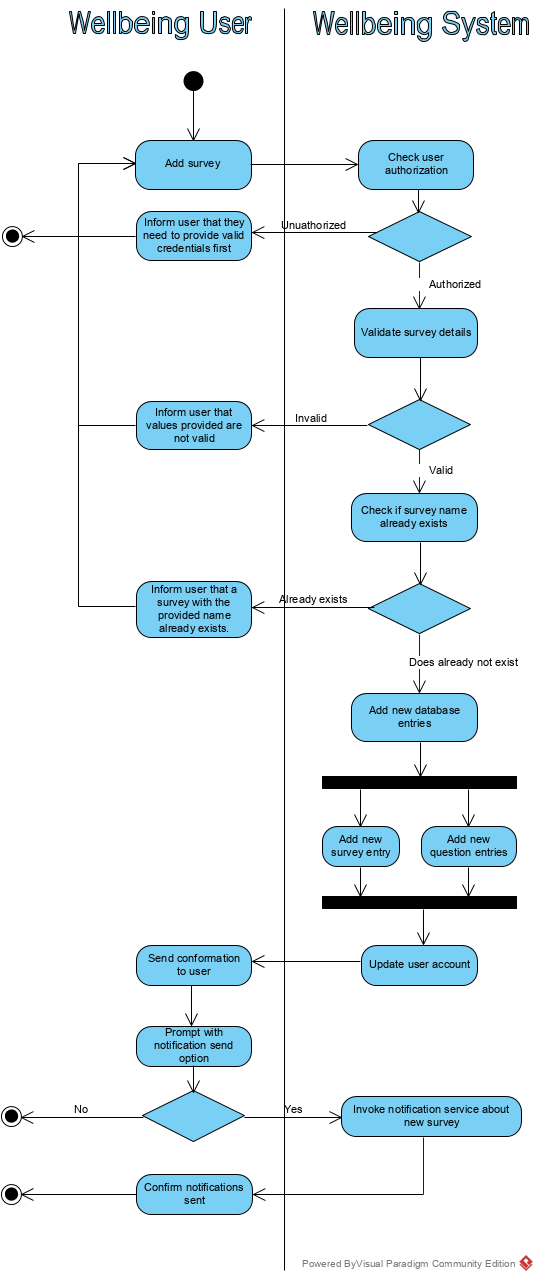
\includegraphics[width=150px]{images/flow_diagram.png}
    \caption{Flow diagram of the processes involved when an \textit{expert} adds a new survey}
\end{figure}

\clearpage

\subsection{REST API}
Talk about the REST api that you have developed in this section.
Give examples, maybe even give 

Maybe list out all the endpoints in a table or something.

\subsection{Database design}

Stuff to do with the database and the database schema.
You can use your JDL thing to represent it here if you really wan to.

\subsubsection{Java Persistence API}
\begin{enumerate}
    \item How entities are defined in the java code 
    \item Talk about JDBC or something as in the way you connected to the database from java
    \item Include the configuration stuff you've also done and explain what it does.
    \item Talk about Repository files and how they act as the interface between the java app and the database
    \item Talk about derrived methods for the repositories
\end{enumerate}


\subsection{Spring security}

Talk about spring security aspects that you have implemented
oauth2 and jwt are good examples
what else?



\subsection{REACT client}
Talk about everything to do with the implementation of the REST client
State how you started off from that OKTA example and worked from there. 

\section{Testing}

To ensure that each component of the application functioned as expected, testing of the entire system is required.
This section will mainly cover user acceptance testing scenarios of the currently implemented features in the software solution.
Potential customers can write acceptance tests to determine if the system is behaving correctly \cite{miller2001acceptance} and 
inherently tests all layers that form the overall architecture.
Acceptance testing also allows the developer to understand if the initial requirements laid out have been met or not.

As of the writing of this report, only the survey management side of the application has been mostly implemented.
This means that, in the application's current state, it behaves more like a generic survey creation tool than something that is specialised
for student wellbeing.
For this reason it is acceptable to form a small group of students from the university to participate in the acceptance testing.
They have been tasked with using the system normally but will also attempt to find faults and cause failures.

\clearpage
\subsubsection{Login page}

 \begin{longtable}{|p{.05\textwidth}|p{.15\textwidth}|p{.15\textwidth}|p{.15\textwidth}|p{.15\textwidth}|p{.05\textwidth}|p{.11\textwidth}|}
  \hline
  ID          &   Test name            & Test                                                                                           & Acceptance \par criteria                                                                                                           & Actual \par outcome                                                                                                                                        & Pass/\par Fail & Comments\\
  \hline\hline                                                                                                                             
  LP1 & Login with invalid credentials & The user is presented with an error                                                            & The user is not redirected to another page. \par Username and password fields are emptied. \par An error is presented to the user. & The system told the user that their credentials were bad. \par System reset username and password fields for them to fill in their credentials again.      & Pass           &         \\
  \hline                                                                                                                                   
  LP2 & Login with no credentials      & The user is presented with an error                                                            & The user is not redirected to another page. \par Username and password fields are emptied. \par An error is presented to the user. & The system told the user that their credentials were bad. \par System reset username and password fields for them to fill in their credentials again.      & Pass           &         \\
  \hline
  LP3 & Login with valid credentials   & The user successfully logs in with the provided credentials and is redirected to the dashboard & The user is able to successfully log into the application with their credentials and is redirected to the dashboard.               & The system accepted their credentails and redirected the user to the dashboard.                                                                            & Pass           &         \\
  \hline
  LP4 & Logout of the system           & Use the logout button to revoke current authentication and be redirected to the login page     & The user is sent back to the login page and cannot go back to the dashboard                                                        & User is sent back to the login page and cannot access any other part of the system                                                                         & Pass           &         \\     
  \hline
\end{longtable}

\subsubsection*{Comments}
Users were satisfied with the overall implementation of the login page and were unable to find any major flaws.
They also appreciated the clean presentation and how credential autocomplete was also compatible with it.

\subsubsection{Survey list page}

\begin{longtable}{|p{.05\textwidth}|p{.15\textwidth}|p{.15\textwidth}|p{.15\textwidth}|p{.15\textwidth}|p{.05\textwidth}|p{.11\textwidth}|}
  \hline
  ID  & Test name                                       & Test                                                                                                                                                                  & Acceptance \par criteria                                                    & Actual \par outcome                                                                                                                 & Pass/\par Fail & Comments\\
  \hline\hline                                                                                                                          
  SL1 & User can view list of surveys they have created & Click on survey manager button from dashboard and user should be redirected to the survey manager page where they will see a list of surveys they have created        & User is redirected to the survey manager page and can see all their surveys & User was successfully transferred to the survey manager page and was able to see all their surveys                                  & Pass           &         \\ 
  \hline
  SL2 & Add a new survey                                & The user is redirected the Add Survey page                                                                                                                            & The user is successfully redirected to the Add Survey page                  & The user was redirected to the Add Survey page where they could entier details for the question name and description before saving. & Pass           &         \\
  \hline                                                                                                                                                                                                                                 
  SL3 & Edit an existing survey                         & The user is redirected to the Edit Survey page                                                                                                                        & The user is successfully redirected to the Edit Survey page                 & The user was redirected to the Edit Survey page where they could alter survey details                                               & Pass           &         \\
  \hline
  SL4 & Displaying delete prompt                        & Clicking the delete button against the survey created in SL2 and making sure a confirmation prompt is shown                                                           & Delete survey confirmation prompt shown                                     & The confirmation prompt for deleting a survey is shown                                                                              & Pass           &          \\ 
  \hline
  SL5 & Delete an existing survey                       & Following on from SL4 confirm deletion for the survey created in SL2                                                                                                  & The survey created in test SL2 is removed from the survey list              & The survey created in test SL2 is no longer present in the survey list                                                              & Pass           &          \\
  \hline
\end{longtable}

\subsubsection*{Comments}
Overall, users were happy with the way the survey list page has been implemented.
The noted how the page was presented in a very clear manner and were easily able to add, edit and delete surveys. 
  
\subsubsection{Survey edit page}


\begin{longtable}{|p{.05\textwidth}|p{.15\textwidth}|p{.15\textwidth}|p{.15\textwidth}|p{.15\textwidth}|p{.05\textwidth}|p{.11\textwidth}|}
  \hline
  ID  & Test name                          & Test                                                                                                                                          & Acceptance \par criteria                                                                                                                                                               & Actual \par outcome                                                                                                                                                       & Pass/\par Fail & Comments\\
  \hline\hline                                                                                                                                                                                                                                                                                                    
  SE1 & Add a new survey                   & Click the Add Survey button, provide a name with description and save it                                                                      & User is sent back to the survey list with the new survey they added now present in the list                                                                                            & User was sent back to the survey list page and their survey was added to the list                                                                                         & Pass           &         \\ 
  \hline                                                                                                                  
  SE2 & Open survey editor for a survey    & Click on the edit button for the survey added in SE1 and user will be redirected to the survey edit page with all the survey details present  & User is sent to the survey edit page with all the survey details for the survey added in SE1 prsent                                                                                    & User was redirected to the survey edit page with all the fields filled with the details provided when creating the survey added in SE1                                    & Pass           &         \\
  \hline                              
  SE3 & Change the survey name             & Change the survey name for the survey created in SE1                                                                                          & User changes the survey name and presses the save button. User is then redirected back to the survey list page with the new survey name applied to the edited survey                   & User applied a new named to the survey and submitted the changes. They were sent back to the survey list page where the new name applied was reflected in the list        & Pass           &         \\  
  \hline                      
  SE4 & Change the survey description      & Change the survey description for the survey created in SE1                                                                                   & User changes the survey description and presses the save button. User is redirected back to the survey list page with the new survey description applied to the survey                 & User applied a new description to the survey and submitted the changes. They were sent back to the survey list page where the new name applied as reflected in the list   & Pass           &         \\
  \hline                        
  SE5 & Change survey name and description & Change both the survey name and description for the survey created in SE1                                                                     & User changes survey name and descrption and presses the save button. User is redirected back to the survey list page with both values being changed to the ones the user had submitted & User changed both name and desciption for the survey and submitted. They were sent back to the survey list page where the new values were shown against the edited survey & Pass           &         \\   
  \hline     
\end{longtable}

\subsubsection*{Comments}
Users encountered no problems with editing surveys, was very straightforward with everything being very clearly presented.

\subsubsection{Survey question editing}

\begin{longtable}{|p{.05\textwidth}|p{.15\textwidth}|p{.15\textwidth}|p{.15\textwidth}|p{.15\textwidth}|p{.05\textwidth}|p{.11\textwidth}|}
  \hline
  ID  & Test name                          & Test                                                                                                                                          & Acceptance \par criteria                                                                                       & Actual \par outcome                                                                                                                                                     & Pass/\par Fail & Comments                                                                   \\
  \hline\hline                                                                                                                                                                                                                                                                              
  QE1 & Add a new survey                   & Click the Add Survey button, provide a name with description and save it                                                                      & User is sent back to the survey list with the new survey they added now present in the list                    & User was sent back to the survey list page and their survey was added to the list                                                                                       & Pass           &                                                                            \\ 
  \hline                                                                                            
  QE2 & Open survey editor for a survey    & Click on the edit button for the survey added in SE1 and user will be redirected to the survey edit page with all the survey details present  & User is sent to the survey edit page with all the survey details for the survey added in SE1 prsent            & User was redirected to the survey edit page with all the fields filled with the details provided when creating the survey added in SE1                                  & Pass           &                                                                            \\
  \hline        
  QE3 & Add a new question with no choices & Attempt to add a new question with no question choices to the survey                                                                          & The question with no choices is added to the survey and can be viewed in the question list                     & The question with no choices is added to the survey and can be viewd in the questions list on the same page                                                             & Pass           & User feels this should not be allowed to happen                            \\
  \hline  
  QE4 & Add an empty question              & Attempt to add a new question with no name or choices                                                                                         & Empty question is not submitted or added to the question list                                                  & Question was not added to the list and refreshing the page did not load it in either                                                                                    & Pass           & User believes an error should be shown to them as more effective feedback  \\               
  \hline  
  QE5 & Add a question with choices        & Attempt to add a new question with at least one choices                                                                                       & The question is submitted and the question, with choices, is displayed in the list                             & The question and its choices were added to the question list and refreshing the page loaded them in again                                                               & Pass           &                                                                            \\
  \hline  
  QE6 & Edit a question choice             & Edit a question choice from the question added in QE5                                                                                         & Change a value in one of the question choices and submit. Value in the question list should also be updated    & The question choice that was edited was successfully submitted and value in the question list was updated. Force reload confirmed value was submitted to server         & Pass           &                                                                            \\        
  \hline  
  QE7 & Add an empty question choice       & Add a new question choice to question but leave one or more of the fields blank                                                               & The question choice with one or more empty fields is not added to the questions or listed in the question list & Submitting a question choice with one or more empty fields led to an exception thrown, crashing the client                                                              & Fail           & Error handling not present for this test scenario                          \\
  \hline
  QE8 & Delete an existing question choice & Delete a question choice that already exists under a question                                                                                 & Question is deleted from the question and is no longer listed in the question list                             & Question is successfully deleted and has been removed from the question list. Reloading the page confirmed that it was no longer being loaded from the server           & Pass           &                                                                            \\
  \hline    
\end{longtable}
 
\subsubsection*{Comments}
For adding and editing questions to the survey, users found it intuitive while maintaining simplicity of use.
When adding a new question without any choices, a couple users noted that they did not believe this should be allowed by the system.
They believed that an error message should be presented to the user telling them they need at least two question choices.
An attempt was made by more than one user to add a new question with no question name but include choices. 
The outcome for this attempt was that nothing happened and the question add window was closed.
Feedback for this particular behaviour was that there should be some sort of feedback to the user to confirm that the question was not added
or that they performed and illegal action.
Question editing raised one system failure when attempting to add a question with one or more empty field. 
Users who had encountered it strongly suggested this needs to be fixed as they found they needed to go back to the login page and navigate 
back to the survey edit page.


\subsubsection{Further feedback}

\subsubsection*{Login page}
There was confusion with why users had to use a provided set of credentials to log into the system as they wanted to be able to register a new account.
This is due to there not being enough development time to implement such a feature.

\subsubsection*{Survey list page}
One feature that was suggested, to be included in the future, is the ability to categorise surveys based on a particular topic or keyword.

\subsubsection*{Survey question editing}
One user suggested that questions should be editable directly from the question list rather than having to use a window.
This suggestion was actually a desire for the developer but was not implemented due to the complexities involved.

\subsubsection*{Testing conclusions}
The use of acceptance testing has proven to be very successful.
In software development not all scenarios are always considered and this is apparent with the tests users had carried out due to the one failure 
found.
Feedback provided by the users in the test group has been very valuable due to the type of quality of life improvements that would benefit users.
When the number of survey becomes large enough, it would be really difficult for users to sort through. 
Though this was never in the general scope of the project, the developer can see the potential value this has.
Originally when developing the question lists, there was a desire to have all the questions be directly editable from the list itself rather than
having to open a new window. 
The developer agrees that this could provide a better experience to users however had to resort to the currently implemented solution due to the 
large complexities encountered during development.

Considering that not all features have been implemented yet, the ones that have have proven to be fit for purpose.
Users were overall pleased with the performance and presentation that was provided by the application.
\section{Dicussion: Contribution and Reflection}
\section{Social, Legal, Health \& Saftety and Ethical Issues}


\bibliographystyle{ieeetr}
\bibliography{bibliography/references}

\end{document}